\documentclass[crop]{standalone}
\usepackage{tikz}
\usepackage{pgfplots}
\usepackage[]{tkz-euclide}
\usetkzobj{all}
\pgfplotsset{compat=1.15}
\usepackage[]{amsmath}
\usepackage[]{libertine}
\usepackage[libertine]{newtxmath}
\usepackage[]{bm}
\usepackage[]{physics}
% Typographical refinement
\usepackage[activate={true,nocompatibility},% Let microtype do its magic
%                                           % without trying to keep page breaks
%                                           % etc.
final=true,% Activate microtype even when in draft mode
kerning=true,% Fixes kerning issues
spacing=true,% Fixes spacing issues
tracking=true,% Adds letter spacing for small caps
shrink=30,% Characters are stretched or shrunk in order to improve justification
stretch=30,% up to 3 %
factor=0% Controls how much punctuation protrudes past the end of the line
]{microtype}
\microtypecontext{spacing=nonfrench} % <-- No spacing found for Linux Libertine
% Macros for greek letters in roman style, in math mode
\DeclareRobustCommand{\mathup}[1]{%
\begingroup\ensuremath\changegreek\mathrm{#1}\endgroup}
\DeclareRobustCommand{\mathbfup}[1]{%
\begingroup\ensuremath\changegreek\bm{\mathrm{#1}}\endgroup}


\makeatletter
\def\changegreek{\@for\next:={%
        alpha,beta,gamma,delta,epsilon,zeta,eta,theta,iota,kappa,lambda,mu,nu,%
        xi,pi,rho,sigma,tau,upsilon,phi,chi,psi,omega,varepsilon,varpi,%
    varrho,varsigma,varphi}%
\do{\expandafter\let\csname\next\expandafter\endcsname\csname\next up\endcsname}}
\makeatother

% Define vectors in bold, roman, lowercase font
\newcommand{\vct}[1]{\ensuremath{\mathbfup{\MakeLowercase{#1}}}}

% Define unit vectors in bold, roman, lowercase font, with hats
\newcommand{\uvct}[1]{\ensuremath{\mathbfup{\hat{\MakeLowercase{#1}}}}}

% Define matrices in bold, roman, uppercase font
\newcommand{\mtrx}[1]{\ensuremath{\mathbfup{\MakeUppercase{#1}}}}
\usetikzlibrary{%
    shapes,%
    arrows,%
    positioning,%
    intersections,%
    calc%
}

\tikzset{
    block/.style = {draw, rectangle, stroke = black!80,fill = gray!15, minimum height = 3em, minimum width = 6em},
    arr/.style = {single arrow, draw, ->}
}
\begin{document}
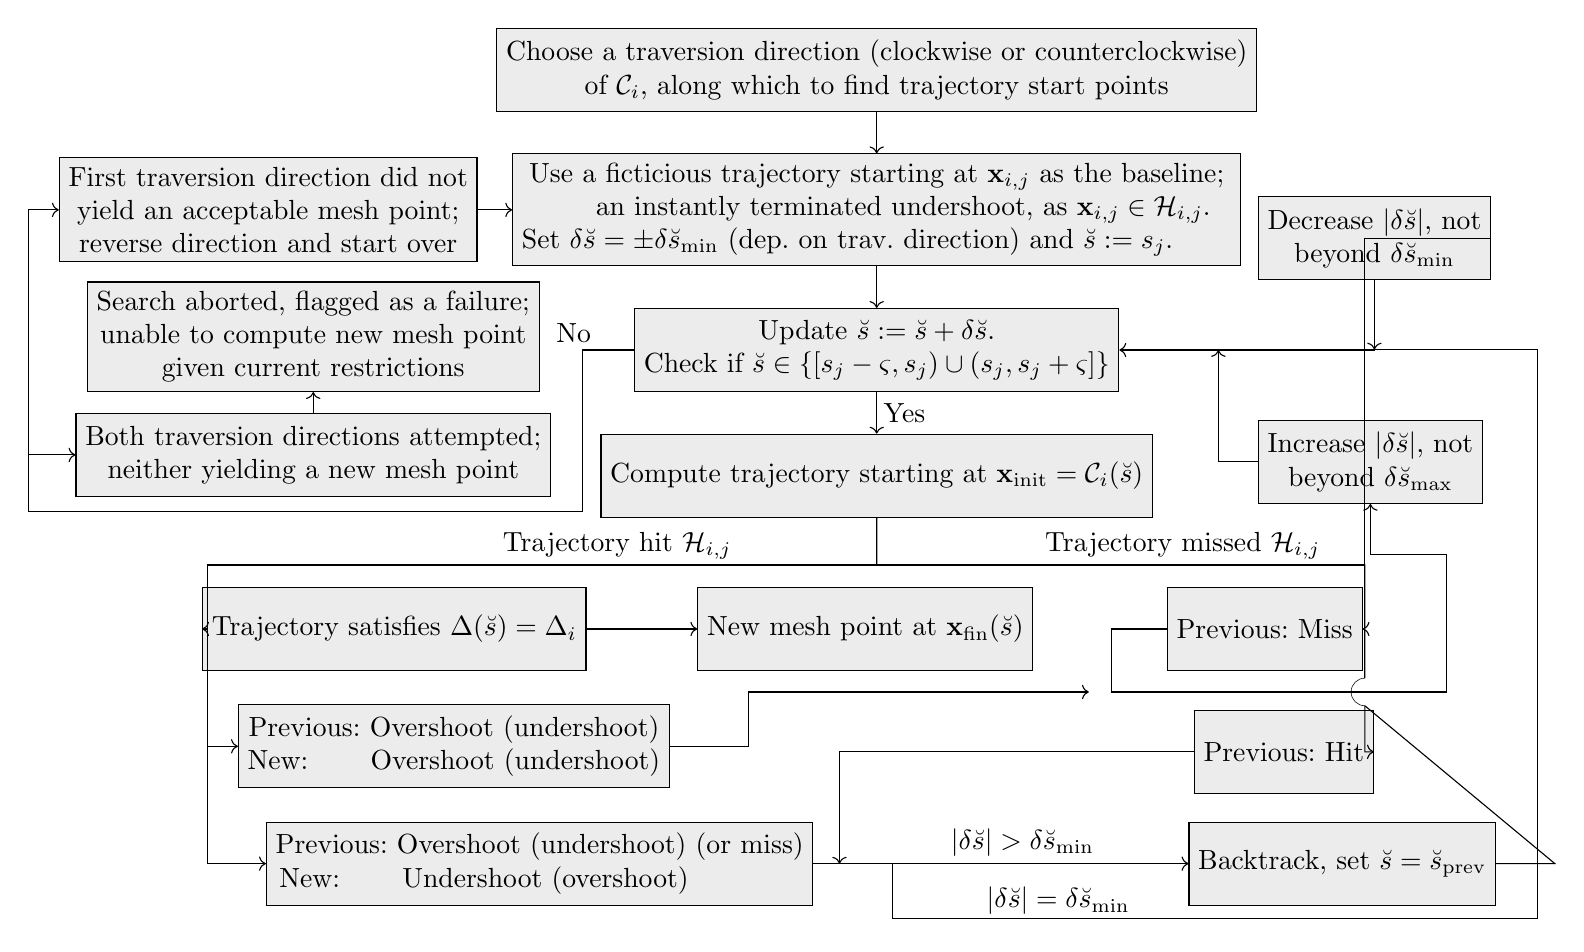
\begin{tikzpicture}
    \node[align=center] (top) [block] {Choose a traversion direction (clockwise or counterclockwise) \\of $\mathcal{C}_{i}$, along which to find trajectory start points};
    \node[align=center, below = 15pt of top] (ficticious) [block] {
            Use a ficticious trajectory starting at $\vct{x}_{i,j}$ as the
            baseline; \\
            \phantom{xxx} an instantly terminated undershoot, as
            $\vct{x}_{i,j}\in\mathcal{H}_{i,j}$. \\ Set
    $\delta\breve{s}=\pm\delta\breve{s}_{\text{min}}$ (dep. on trav.
    direction) and
$\breve{s}:=s_{j}$.\phantom{xxxx}};
    \node[align=center, below = 15pt of ficticious] (flipcheck) [block] {Update
         $\breve{s}:=\breve{s}+\delta\breve{s}$.\\Check if $\breve{s} \in \{[s_{j}-\varsigma,s_{j})\cup(s_{j},s_{j}+\varsigma]\}$};
    \node[align=center, below left = 7.5pt and 30pt of flipcheck] (flipboth)
        [block] {Both traversion directions attempted;\\ neither yielding a new
        mesh point};
    \node[align=center, above = 7.5pt  of flipboth] (flip-terminate) [block]
        {Search aborted, flagged as a failure; \\unable to compute new mesh point\\ given current restrictions};
    \node[align=center, left = 12.5pt of ficticious] (flipone) [block]
        {First traversion direction did not\\ yield an acceptable mesh point;\\
            reverse direction and start over};
    \node[align=center, below = 15pt of flipcheck] (launch) [block] {Compute trajectory starting at $\vct{x}_{\text{init}} = \mathcal{C}_{i}(\breve{s})$};

    \node[align=center, above right =10pt and 50pt of flipcheck] (decrease-right) [block] {Decrease $\abs{\delta\breve{s}}$, not\\ beyond $\delta\breve{s}_{\min}$};
    \node[align=center, below right = 10pt and 50pt of flipcheck] (increase-right) [block] {Increase $\abs{\delta\breve{s}}$, not\\ beyond $\delta\breve{s}_{\max}$};

    \node[align=center, below left = 25pt and 5pt of launch] (accepted) [block] {Trajectory satisfies $\Delta(\breve{s})=\Delta_{i}$};
    \node[align=center, below right = 12pt and -126pt of accepted] (hit-prevhit) [block] {Previous: Overshoot (undershoot)\\New: \phantom{xxx} Overshoot (undershoot)};
    \node[align=center, below right = 12pt and -146pt of hit-prevhit] (hit-prevmiss) [block] {Previous: Overshoot (undershoot) (or miss)\\New: \phantom{xxx} Undershoot (overshoot) \phantom{xxxxxxx}};


    \node[align=center, right = 40pt of accepted] (exit-success) [block] {New mesh point at $\vct{x}_{\text{fin}}(\breve{s})$};

    \node[align=center, below right = 25pt and 5pt of launch] (miss-prevhit) [block] {Previous: Miss};
    \node[align=center, below right = 14pt and -61pt of miss-prevhit](miss-prevmiss) [block] {Previous: Hit};
    \node[align=center, below right = 10pt and -67pt of miss-prevmiss] (backtrack-miss) [block] {Backtrack, set $\breve{s}=\breve{s}_{\text{prev}}$};

    \draw[arr] (top.south) -- (ficticious.north);
    \draw[arr] (ficticious.south) -- (flipcheck.north);
    \draw[arr] (flipcheck.south) -- (launch.north) node [auto, swap, xshift =
        10, yshift = 7.5] {Yes};
    \draw[arr] (flipcheck.west) -- ++(-0.65,0) -- ++(0,-2.05) -|
        ($(flipboth.west)-(0.6,0)$) |- (flipboth.west) node [auto, swap, xshift = 180, yshift = 44] {No};
    \draw[arr] (flipboth.west) --++(-0.6,0) --++(0,3.) |- (flipone.west);
    \draw[arr] (flipboth.north) -- (flip-terminate.south);
    \draw[arr] (accepted.east) -- (exit-success.west);

    \draw[arr] (launch.south) -- ++(0,-0.6) -- ++(6.2,0) -- ++(0,-0.81) |- (miss-prevhit.east) node [auto, swap, xshift = -65, yshift = 30] {Trajectory missed $\mathcal{H}_{i,j}$};
    \draw[arr] (launch.south) -- ++(0,-0.6) -- ++(-8.5,0) -- ++(0,-0.81) |- (accepted.west) node [auto, swap, xshift = 150, yshift = 30] {Trajectory hit $\mathcal{H}_{i,j}$};
    \draw[arr] (launch.south) -- ++(0,-0.6) -- ++(-8.5,0) -- ++(0,-2.23) |- (hit-prevhit.west);
    \draw[arr] (launch.south) -- ++(0,-0.6) -- ++(-8.5,0) -- ++(0,-3.65) |- (hit-prevmiss.west);
    \draw[arr] (flipone.east) -- (ficticious.west);

    \draw[arr] (hit-prevhit.east) -- ++(1,0) --++(0,0.69) -- ++(4.32,0);

    \draw[arr] (hit-prevmiss.east) -- (backtrack-miss.west) node [auto, swap,
    xshift = -60, yshift = 7.5]
    {$\abs{\delta\breve{s}}>\delta\breve{s}_{\min}$};
    \draw[arr] (miss-prevmiss.west) -- ++(-0.5,0) -- ++(-4,0) --
    ++(0,-1.42);
    % Define start and end points for path 1 (downwards)
    \coordinate (p0) at ($(launch.south) +(0,-0.6) +(6.2,0) + (0,-0.81)$);
    \coordinate (p1) at ($(p0)+(0,-1.425)$);

    % Compute path 1
    \path[name path=line 1] (p0)--(p1);


    % Draw path 2
    \draw[arr,name path = line 2] (miss-prevhit.west) -- ++(-0.7,0) --
    ++(0,-0.8) -- ++(4.25,0) -- ++(0,1.75)  -| (increase-right.south);

    % Find intersection of first and second paths
    \path[name intersections={of = line 1 and line 2}];
    \coordinate (S) at (intersection-1);
    % Path a circle around this intersection for the arc
    \path[name path = circle] (S) circle(5pt);

    % Find intersections of first line and circle
    \path[name intersections={of = circle and line 1}];
    \coordinate (I1) at (intersection-1);
    \coordinate (I2) at (intersection-2);

    % Draw normal line segments
    \draw (launch.south) -- ++(0,-0.6) -- ++(6.2,0) -- (p0) -- (I1);
    \draw[arr] (I2) -- (p1) |- (miss-prevmiss.east);
    \tkzDrawArc[color=black](S,I1)(I2);

    \draw[arr] (decrease-right.south) |- (flipcheck.east);
    \draw[arr] (decrease-right.south) -- ++(0,-0.88);
    \draw[arr] (increase-right.west) -- ++(-0.5,0) -- ++(0,1.42) ;

    % Draw main line segment
    \draw (hit-prevmiss.east) -- ++(1.,0) -- ++(0,-0.7) -- ++(8.2,0) --
    ++(0,7.225) coordinate (q1);
    \node[auto, below right = 5pt and -187.5pt of backtrack-miss.east]
    {$\abs{\delta\breve{s}}=\delta\breve{s}_{\min}$};
    \coordinate (q2) at ($(q1)+(-5,0)$);
    % Compute path 1
    \path[name path = line 1] (q1)--(q2);

    % Draw path 2
    \path[name path = line 2] (backtrack-miss.east) -- ++(0.75,0) |- (decrease-right.east);

    % Find path intersections
    \path[name intersections={of = line 1 and line 2}];
    \coordinate (S) at (intersection-1);
    % Path a circle around this intersection for the arc
    \path[name path = circle] (S) circle(5pt);
    % Find intersections of first line and circle
    \path[name intersections={of = circle and line 2}];
    \coordinate (I1) at (intersection-1);
    \coordinate (I2) at (intersection-2);

    % Draw normal line segments
    \draw (q1) -- (q2);
    \draw (backtrack-miss.east) -- ++(0.75,0) -- (I2);
    \draw (I1) |- (decrease-right.east);
%    \draw (q1) -- (I1);
%    \draw (I2) -- (q2);
    \tkzDrawArc[color=black](S,I1)(I2);




\end{tikzpicture}
\end{document}
